\section{Methods}
\label{sec:methods}
We begin this section with an overview of our experimental design. Then we introduce the objective functions that we used to compute MSA. Finally, we discuss the multi-objective metaheuristics applied to optimize those objective functions as well as the state-of-the-art tools that we utilized in this study. Because we deal with a number of objective functions, more than 10 state-of-the-art MSA tools and more than 30 instances of MSA problem, a reader is exposed to an over-preponderance of acronyms and short-cut notations. Therefore, for the sake of ease in exposition and understanding, we alphabetically list all the acronyms used in this study with their usage in Table~\ref{tab:acronyms} of the supplementary file.
%Afterwards, we describe our method of evaluating estimated alignments and phylogenetic trees. Finally, we summarize the methodology followed to establish the effectiveness of our objectives. 

\begin{figure}[!htbp]
	\centering
	%\begin{adjustwidth}{-0.5cm}{-0.5cm}
	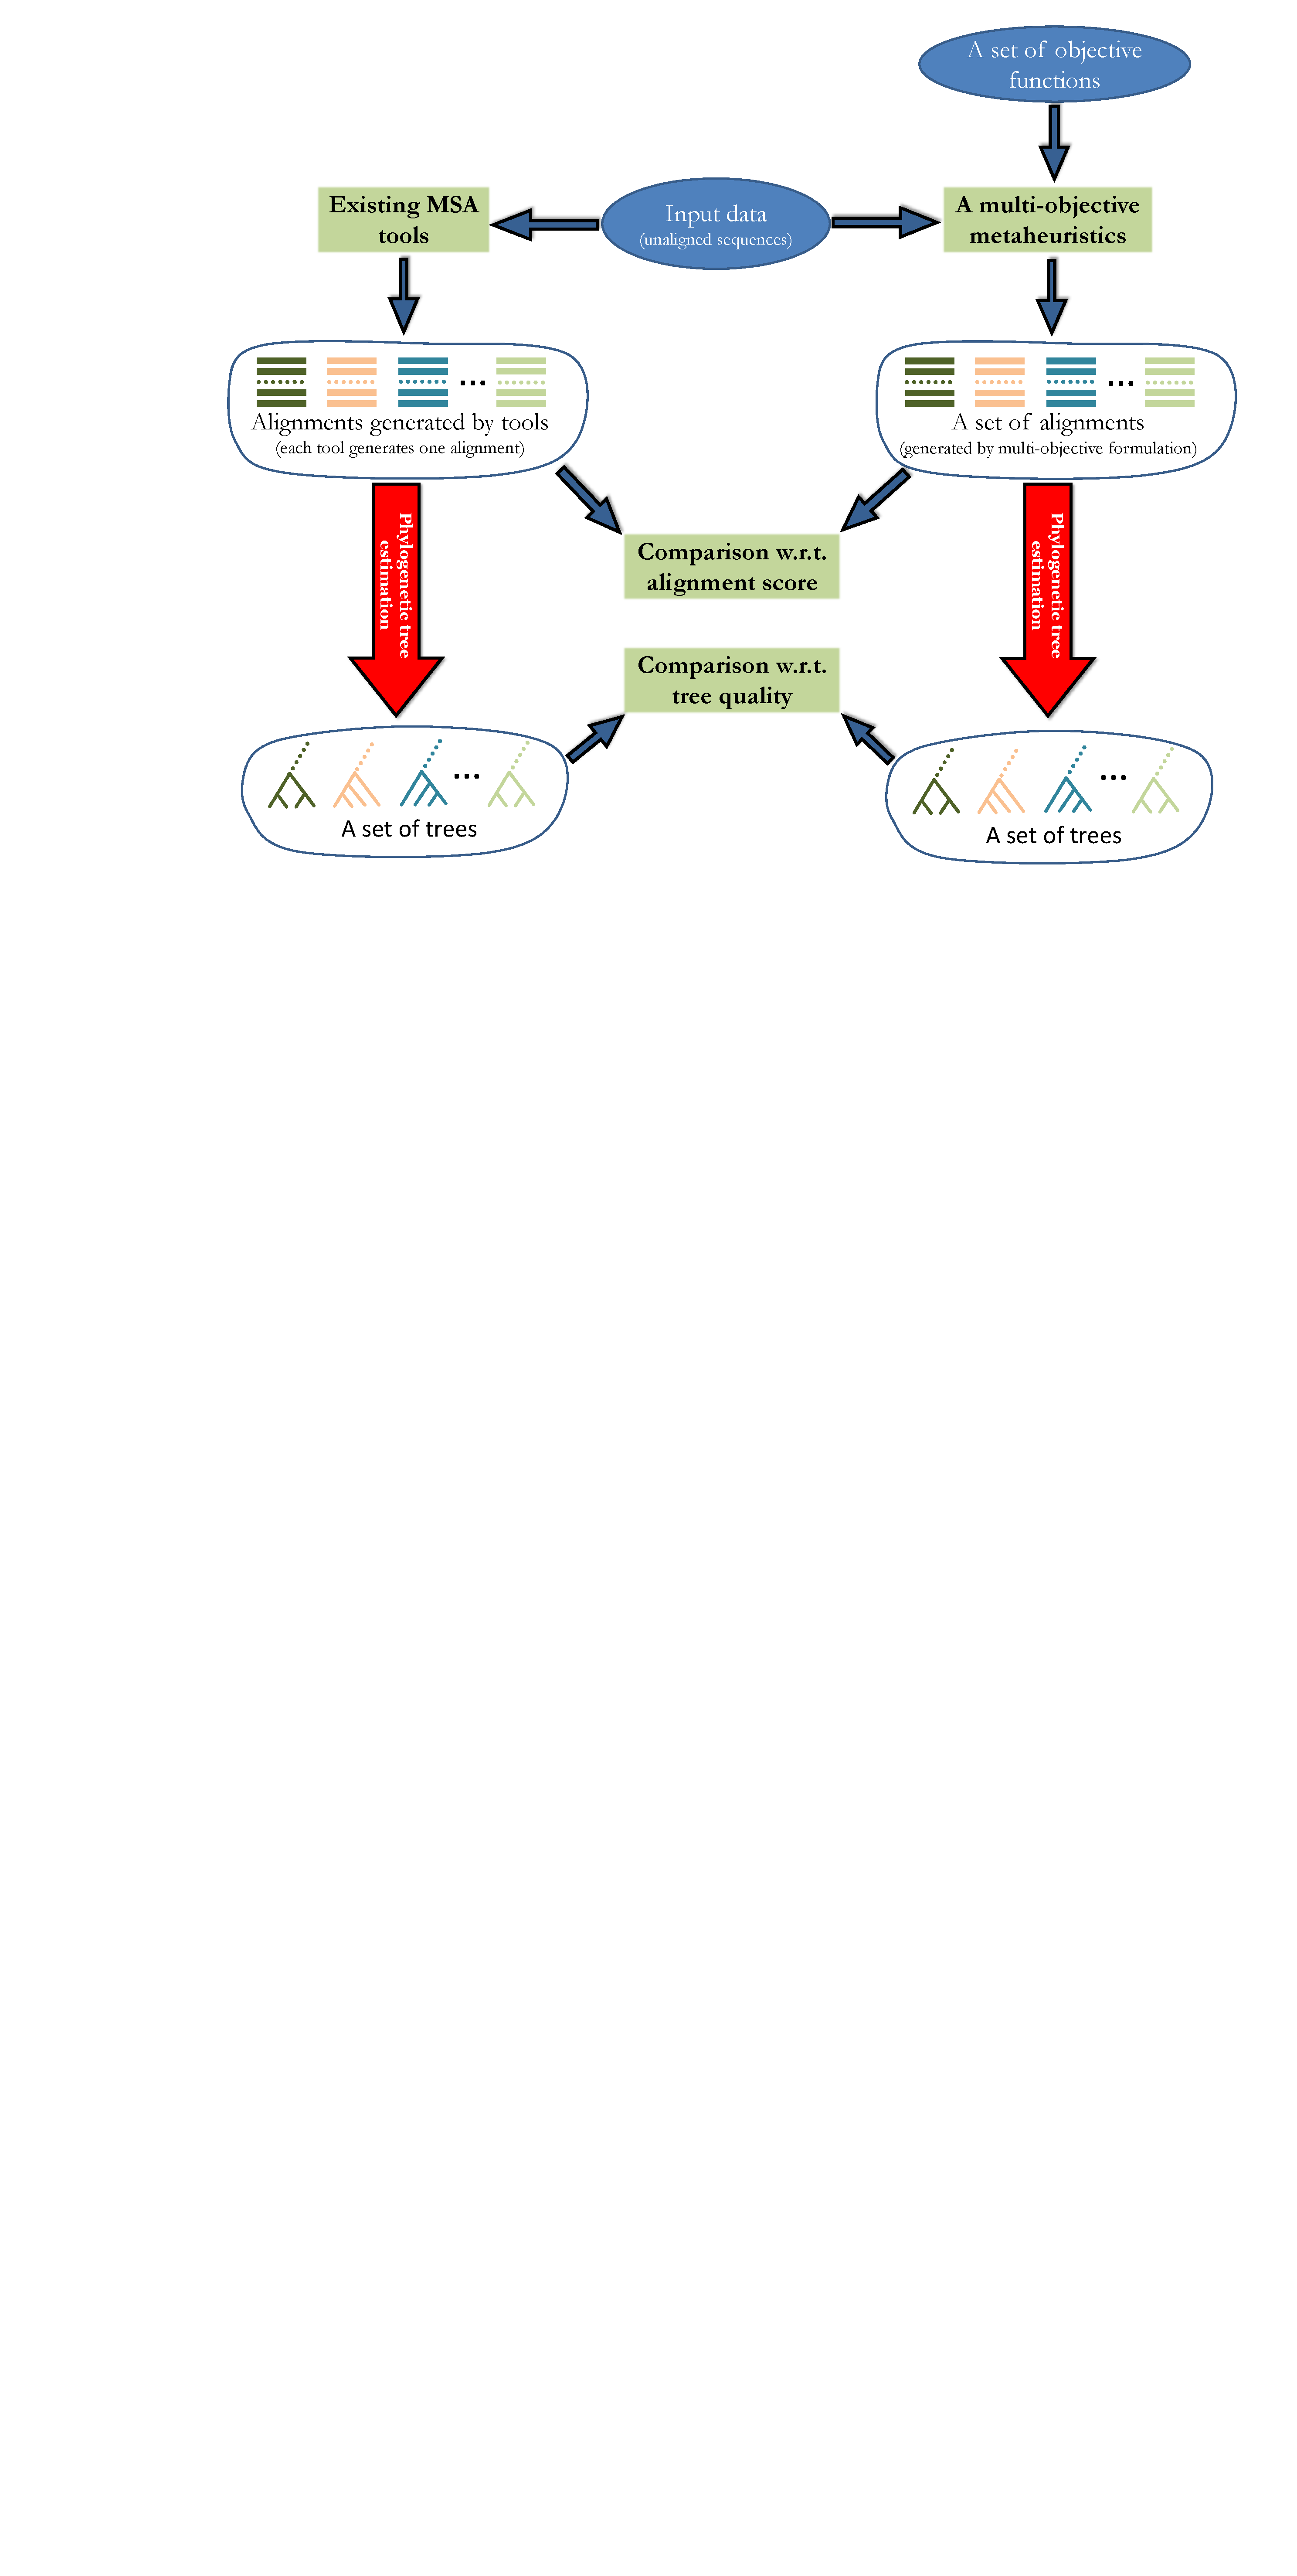
\includegraphics[width=0.5\textwidth]{Figure/pipeline}
	\caption{Our methodology for finding the impact of a multi-objective formulation (i.e., a set of objective functions) of MSA on phylogenetic tree estimation.} 
		%For each dataset (i.e., unaligned sequences), we run a multi-objective metaheuristic. It simultaneously optimizes the given objective functions and outputs a set of alignments which represents the best-possible compromise among all objective functions. We also run several existing MSA tools on that dataset and each tool generates one alignment. We evaluate the quality of each generated alignments with respect to the reference alignments using widely used scores. Also, we estimate phylogenetic trees for all alignments and evaluate each tree with respect to the reference. Then we compare the alignments and the corresponding phylogenetic trees generated by the multi-objective formulation with the ones generated by the existing tools based on alignment score as well as tree quality. We also observe the association between alignment scores and tree quality values to examine whether it is appropriate to use alignment score in the context of phylogeny estimation.
	\label{fig:pipeline}
	%\end{adjustwidth}
\end{figure}

\subsection{Experimental design}
Our experimental methodology is briefly described below (please see also Figure~\ref{fig:pipeline}):
\begin{itemize}
	\item \underline{Step 1:} Following a systematic approach involving multiple linear regression applied on a simulated dataset, we first make an attempt to identify and choose two multi-objective formulations that turn out to be potentially more effective in the context of phylogeny estimation (discussed in Section~\ref{sec:obj_eval} of the supplementary file). 
	\item \underline{Step 2:} We run a popular and effective multi-objective metaheuristics on biological datasets to optimize each set of objective functions selected in Step 1. Each run of the metaheuristics on each dataset gives us a set of alignments as the final output. 
	\item \underline{Step 3:} We also run nine state-of-the-art MSA tools (please see Table~\ref{tab:msa_tools}) to generate alignments on all these datasets.
	% \comment{with default parameters. It is the usual practice of MSA literature. Should I exclude this?} and then estimate maximum likelihood (ML) phylogenetic tree from those alignments. We evaluate the quality of these alignments and ML trees.
	\item \underline{Step 4:} We evaluate the quality of each generated alignment with respect to the reference alignment using two popular measures, namely, SP score and TC score (discussed in Section~\ref{sec:msa_eval} of the supplementary file). 
	%For biological datasets, we used manually curated alignments as reference.
	\item \underline{Step 5:} For each of the generated alignments, we infer maximum likelihood (ML) phylogenetic tree (discussed in Section~\ref{sec:tree_estimation} of the supplementary file). Then we measure the quality of each inferred tree with respect to the reference tree (true tree) using a commonly used measure in the literature called false negative (FN) rate~\citep{warnow2017computational} (discussed in Section~\ref{sec:tree_eval} of the supplementary file).
	\item \underline{Step 6:} Finally we compare the alignments and the corresponding ML trees generated by the multi-objective optimization with the ones generated by the state-of-the-art tools. % using statistical measures.
\end{itemize}

\subsection{Objective functions}
\label{sec:formulation}
Most real-world optimization problems naturally work towards achieving several objectives. Some of these objectives are conflicting to each other. However, these problems can be transformed into single-objective ones using various simplifying techniques to avoid complexities~\citep{kalyanmoy2001multi}. On the contrary, a multi-objective formulation defines the problem using a set of objective functions and subsequently specialized methods can be applied to optimize all the objectives simultaneously. In this study, we have selected the following three multi-objective formulations of MSA from the literature based on their simplicity as well as performance as reported in the literature.
\begin{itemize}
	\item \{SOP, TC\}: Maximize the sum of pairs (SOP) and the number of totally aligned columns (TC)~\citep{da2010alineaga}.
	
	\item \{Gap, SOP\}: Maximize the sum of pairs (SOP) and minimize the number of gaps (Gap)~\citep{abbasi2015local}.
	
	\item \{wSOP, TC\}: Maximize the weighted sum of pairs with affine gap penalties (wSOP) and the number totally aligned columns (TC)~\citep{rubio2016hybrid}.
\end{itemize}

We describe these objective functions along with several existing ones in Section~\ref{sec:objective _function} of the supplementary file. Now, we propose four new objective functions that quantify different aspects of an MSA. Unlike the existing objective functions in the literature, we avoid combining multiple aspects of an MSA into a single objective. We introduce them as follows: 

\begin{itemize}
	
	\item \textbf{Minimize entropy (Entropy)}: We modify the usual definition by considering only non-gap column for the calculation of entropy.
	
	\item \textbf{Maximize similarity based on gap containing columns (SimG)}: Here we calculate similarity only for those columns that contain at least one gap. 
	
	\item \textbf{Maximize similarity based on non-gap columns (SimNG)}: We consider only non-gap column while measuring similarity.
	
	\item \textbf{Maximize concentration of gaps (GapCon)}: We find that a widely used objective function, namely, affine gap penalty~\citep{rani2016multiple}, combines two aspects of an aligned sequence, number of gaps and concentration of gaps, into a single one using weighted sum. We need to tune the weight values based on the dataset. To avoid this tuning we decide to decouple the two components. We have already considered the number of gaps as an objective function. Now we define the concentration of gaps as an independent objective which as calculated as follows. For each sequence, we count the number of consecutive gaps and take the mean of these counts. Finally, we average the resultant means for all sequences.
\end{itemize}

In this study, we used the terms shown in Table~\ref{tab:abbr} to refer to these objective functions. 

% Table generated by Excel2LaTeX from sheet 'abbr'
\begin{table}[!htbp]
	\centering
	%\small
	\caption{Terms used to denote the objective functions.}
	\begin{tabular}{|l|L{6cm}|c|} %{5cm}
		\hline
		\# & \multicolumn{1}{c|}{Objective function} & Term \\
		\hline
		1 & Maximize no. of totally aligned columns & TC \\
		\hline
		2 & Minimize no. of gaps & Gap \\
		\hline
		3 & Maximize sum of pairs & SOP \\
		\hline
		4 & Maximize weighted sum of pairs with affine gap penalties & wSOP \\
		\hline
		5 & Minimize entropy & Entropy \\
		\hline
		6 & Maximize similarity based on gap containing columns & SimG \\
		\hline
		7 & Maximize similarity based on non-gap columns & SimNG \\
		\hline
		8 & Maximize concentration of gaps & GapCon \\
		\hline
	\end{tabular}%
	\label{tab:abbr}%
\end{table}%

\begin{comment}
So, in this study we work run our optimization algorithm with these set of objective function:

\begin{itemize}
\item \{Gap, SOP\}

\item \{SOP, TC\}

\item \{wSOP, TC\}

\item \{Gap, SOP, wSOP, TC\}
\item \{Entropy, TC, Gap, SimG, SimNG, GapCon\}
\item \{SimG, SimNG\}
\end{itemize}
\end{comment}

We need a substitution matrix to calculate SOP and wSOP. The values of this substitution matrix depend on the trait of a particular dataset. In this study, we used NUC4.4 (supplied by NCBI at \url{ftp://ftp.ncbi.nih.gov/blast/matrices/NUC.4.4}) for nucleotide sequences and BLOSUM62~\citep{henikoff1992amino} for protein sequences. On the contrary, the four objective functions that we proposed are nonparametric which are independent of the dataset.

\subsection{Multi-objective metaheuristics} %Multi-objective Metaheuristics Generation of competitive alignments
To simultaneously optimize multiple objective functions, we ran two popular multi-objective metaheuristics: NSGA-II~\citep{deb2002fast} and NSGA-III~\citep{deb2014evolutionary}. They belong to the class of multi-objective evolutionary algorithms. They start from a set of candidate solutions (termed as population) and then uses mechanisms inspired by biological evolution (such as mutation, crossover, selection, etc.) to evolve the population towards the optimal solutions. Unlike single-objective optimization methods, they output a set of solutions (i.e. members of the final population)
which represents the best possible compromise of all objectives under consideration. Two studies (\citep{zambrano2017m2align, ortuno2013optimizing}) demonstrated the strength of NSGA-II for solving MSA. NSGA-II works best when the number of objectives is upto three while NSGA-III is specially designed for handling more than three objectives. Hence, we applied these algorithms according to Table~\ref{tab:variants}.
%In this study, we simultaneously optimize two to six objective functions. Therefore, we select these two algorithms to work with. 
We discuss these methods along with their vital components and parameters in Section~\ref{sec:mop} of the supplementary file. We implemented them using jMetalMSA~\citealp{zambrano2017multi} which is a Java metaheuristic framework for MSA. Our implementation is publicly available at \url{https://github.com/ali-nayeem/MSA}.
%Table~\ref{tab:variants}. 
%We implement these two metaheuristics using jMetalMSA of~\citealp{zambrano2017multi} which is a Java metaheuristic framework for MSA publicly available at~\url{https://github.com/jMetal/jMetalMSA}. 
% Table generated by Excel2LaTeX from sheet 'multi-pc'
\begin{table}[!htbp]
	%\small
	\centering
	\caption{Our selected algorithms and corresponding objective set.}
	\begin{tabular}{|c|l|} %{5cm}
		\hline
		Algorithm & Objective set \\
		\hline
		\multicolumn{1}{|c|}{\multirow{4}{*}{NSGA-II}} & \{Gap, SOP\}\\
		& \{SOP, TC\}          \\
		& \{wSOP, TC\} \\
		& \{SimG, SimNG\} \\
		\hline
		\multicolumn{1}{|c|}{\multirow{3}{*}{NSGA-III}} & \{Gap, SOP, wSOP, TC\} \\
		& \{Entropy, TC, Gap, SimG, SimNG, GapCon\} \\
		\hline
	\end{tabular}%
	\label{tab:variants}%
\end{table}%


\subsection{State-of-the-art MSA tools}
We used the alignments generated by nine representative state-of-the-art MSA tools (shown in Table~\ref{tab:msa_tools}) to compare with our approach. We run each of them with its default parameter configuration. Moreover, we initialize the multi-objective metaheuristics with a set of alignments generated by randomly mixing and modifying those nine alignments. Notably, this approach, known as the seeded initial population generation, is quite common in the metaheuristics literature specially for multi-objective optimization. 
%Table~\ref{tab:msa_tools} and Table~\ref{tab:msa_tools} show the list of the MSA tools

% Table generated by Excel2LaTeX from sheet 'single'
\begin{table}[htbp]
	%\small
	\centering
	\caption{List of state-of-the-art MSA tools that we used in this study.}
	\begin{tabular}{|l|l||l|l|}
		\hline
		\multicolumn{2}{|c||}{For nucleotide sequences} & \multicolumn{2}{c|}{For protein sequences} \\
		\hline
		\multicolumn{1}{|c|}{Tool} & \multicolumn{1}{c||}{Version} & \multicolumn{1}{c|}{Tool} & \multicolumn{1}{c|}{Version} \\
		\hline
		FSA~\citep{bradley2009fast} & 1.15.9 & FSA   & 1.15.9 \\
		\hline
		PASTA~\citep{mirarab2015pasta} & 1.7.8 & PASTA & 1.7.8 \\
		\hline
		T-Coffee~\citep{notredame2000t} & 11.00 & T-Coffee & 11.00 \\
		\hline
		MAFFT~\citep{katoh2002mafft} & 7.31  & MAFFT & 7.245 \\
		\hline
		Clustal W~\citep{thompson1994clustal} & 2.1   & Clustal W & 2.1 \\
		\hline
		Clustal $ \Omega $~\citep{sievers2011fast} & 1.2.4 & RetAlign~\citep{szabo2010reticular} & 1.0 \\
		\hline
		MUSCLE~\citep{edgar2004muscle} & 3.8.31 & MUSCLE & 3.8.31 \\
		\hline
		PRANK~\citep{loytynoja2005algorithm} & 0.170427 & ProbCons~\citep{do2005probcons} & 1.12 \\
		\hline
		Kalign~\citep{lassmann2008kalign2} & 2.03  & Kalign & 2.04 \\
		\hline
	\end{tabular}%
	\label{tab:msa_tools}%
\end{table}%

\begin{comment}

\subsection{Evaluation of estimated alignments}
We evaluate estimated alignments with respect to reference alignment using two well-known alignment quality scores called TC score and SP score. These two scores are defined below:
\begin{itemize}
\item TC score is the ratio of the number of correctly aligned columns in the estimated alignment to the total number of aligned columns in the reference alignment. This is also known as column score.

\item SP score is the ratio of the number of aligned pairs in the estimated alignment to the total number of aligned pairs in the reference alignment.

%\item Pairs score is the mean of SP-score and Modeler. SP-Score is the ratio of the number of aligned pairs to the total number of aligned pairs in the reference alignment. And Modeler is very similar to the SP-score where we take the ratio of the number of aligned pairs to the total number of aligned pairs in the estimated alignment      
\end{itemize}
For both the measures, higher value implies better score.

\subsection{Phylogenetic tree estimation}
For each of the generated alignment we estimate the phylogenetic tree using Maximum Likelihood (ML) method. We used a popular tool named FastTree-2 developed by \citealp{price2010fasttree}. %It is publicly available at \url{http://www.microbesonline.org/fasttree/}.

\subsection{Evaluation of phylogenetic tree}
We evaluate the quality of each estimated ML tree with respect to the true phylogenetic tree using a widely used measure known as the False Negative (FN) rate. FN rate is the percentage of edges present in the true tree but missing in the estimated tree. So a small value of FN rate is desirable. %as a quality measure, 

\subsection{Evaluation of objective functions}
In the context of phylogeny estimation, a desired objective function for MSA should lead to such alignments which can produce highly accurate (having small FN rate) ML trees. Considering this fact, we try to evaluate the effectiveness of an objective function by studying how its values are associated with the corresponding FN rates. The objective function that frequently exhibits positive correlation with FN rate is predicted to be a good optimization criteria. To accomplish this, we fit multiple linear regression model to calculate the degree of association (i.e., regression coefficient) between an objective and FN rate. Then we apply t-test, with null hypothesis that there is no association, to check the significance of individual regression coefficients. It should be noted that, such regression results does not necessarily indicate the strength of an objective as an optimization criterion. However, such results can definitely be utilized as the starting point for experimentation for further validation.
%Rather, we expect an objective function, which exhibits larger value compared to others frequently, to guide the optimization algorithms better than other.
\end{comment}
\begin{comment}
\subsection{Computational time}
We ran the multi-objective metaheuristics on a server with Intel(R) Xeon(R) CPU E5-4617 @ 2.90GHz processor and 64GB of RAM. In Table~\ref{tab:time}, we give a rough estimate of the total computational time that we invested to derive our results.

\begin{table}[htbp]
\small
\centering
\caption{Computational time invested to study the impact of multi-objective formualtion of MSA.}
\begin{tabular}{|l|l|}
\hline 
\multicolumn{1}{|c|}{Dataset} & \multicolumn{1}{c|}{Total time (hours)} \\ 
\hline 
100-taxon simulated dataset &  1269.38\\ 
\hline 
Biological rRNA dataset &  311.64\\ 
\hline 
BAliBASE dataset &  45.88\\ 
\hline 
\end{tabular} 
\label{tab:time}%
\end{table}%
\end{comment}